\chapter{Allocation Views}

\section{Deployment Diagram}

\begin{figure}[h]
    \centering
    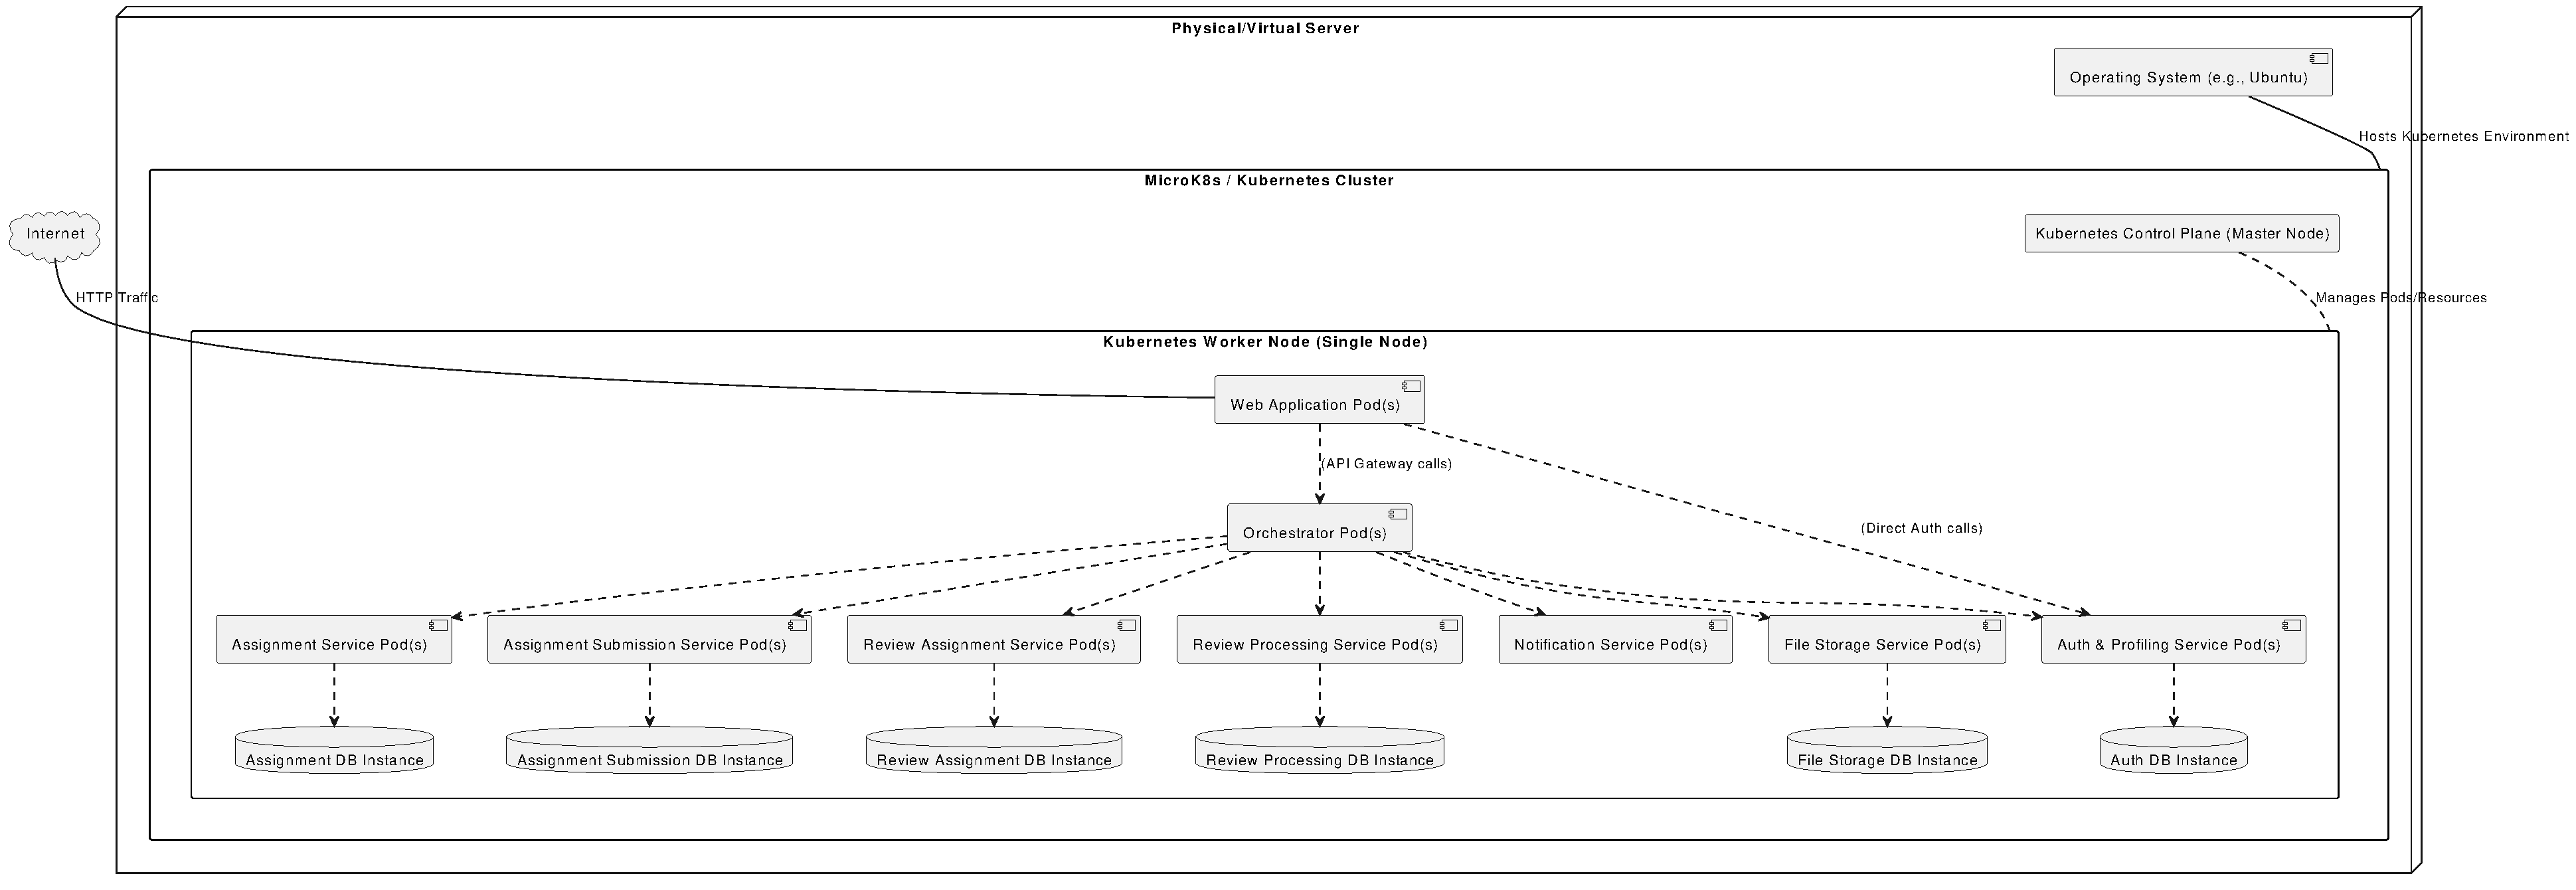
\includegraphics[width=0.9\linewidth]{Architettura/imgs/deploymentview.pdf}
    \caption{Deployment diagram of the system.}
    \label{fig:deploymentViewGlobal}
\end{figure}

\begin{justify}
    The system's deployment architecture is centered around a single Ubuntu Virtual Machine (VM). This VM serves as the host for a single-node Kubernetes cluster, powered by MicroK8s. Within this Kubernetes environment, the entire system is deployed, encompassing the Web Application, an Orchestrator, all defined microservices, and their respective database instances.

    For enhanced scalability and availability, each microservice is deployed as a series of Kubernetes Pods, with more than one replica for each service. This allows the system to handle increased loads and ensures continuous operation even if one instance fails.

    To prevent data inconsistency issues, the database instances themselves are not replicated. Instead, each database instance is designed to manage its own scalability, leveraging technologies like MongoDB, which inherently supports horizontal scalability and fault tolerance. 
    
    The Kubernetes cluster also includes a Master Node, responsible for managing the deployment and lifecycle of the Pods within the cluster.
\end{justify}


\subsection{Rationale}

\begin{justify}
    The decision to deploy PeerFlow on a single-node Kubernetes cluster utilizing MicroK8s on an Ubuntu Virtual Machine was primarily driven by the immediate availability of the resources. This lightweight setup provides a practical environment for demonstrating the system's microservices architecture and core functionalities. However, it is crucial to acknowledge that for a system designed to support a large and highly variable number of users, typical of MOOC environments like Coursera or Udacity, this single-node configuration represents a significant constraint. Ideally, a high-performance, multi-node Kubernetes cluster would be essential. Such a cluster would offer the necessary computational and storage resources, along with enhanced fault tolerance and horizontal scaling capabilities, to effectively manage the demands of potentially millions of concurrent users and a vast amount of data, ensuring optimal performance and availability under peak loads.
\end{justify}
